%%%%%%%%%%%%%%%%%%%%%%%%%%%%%%%%%%%%%%%%%%%%%%%%%%%%%%%%%%%%%
%% HEADERs
%%%%%%%%%%%%%%%%%%%%%%%%%%%%%%%%%%%%%%%%%%%%%%%%%%%%%%%%%%%%%
\documentclass{report}
\usepackage{amsmath}
\usepackage{fullpage}
\usepackage{graphicx}
\usepackage{subfig}
\usepackage{float}
\usepackage{wrapfig}
\usepackage[section]{placeins} 
\graphicspath{ {./../images/} }

\usepackage{color}   %May be necessary if you want to color links

%%%%%%%%%%%%%%%%%%%%%%%%%%%%%%%%%%%%%%%%%%%%%%%%%%%%%%%%%%%%%
%% PARAMS
%%%%%%%%%%%%%%%%%%%%%%%%%%%%%%%%%%%%%%%%%%%%%%%%%%%%%%%%%%%%%
\usepackage{hyperref}
\hypersetup{
    colorlinks=true, %set true if you want colored links
    linktoc=all,     %set to all if you want both sections and subsections linked
    linkcolor=black,  %choose some color if you want links to stand out
}
\author{Clara STAVUN, Anatole MAURER, Charles FARHAT, Haga RANDRIANALY}
\title{Maillage vs nuage de points: analyse comparative}


%%%%%%%%%%%%%%%%%%%%%%%%%%%%%%%%%%%%%%%%%%%%%%%%%%%%%%%%%%%%%
%% DOCUMENT
%%%%%%%%%%%%%%%%%%%%%%%%%%%%%%%%%%%%%%%%%%%%%%%%%%%%%%%%%%%%%
\begin{document}

\maketitle

\tableofcontents


%% Chapters %%%%%%%%%%%%%%%%%%%%%%%%%%%%%%%%%%%%%%%%%%%%%%%%%
%% Chaque chapitres sont dans un fichier

%% Contient le chapitre sur l'étude comparative entre les deux méthodes

\chapter{Etude comparative Nuages de points et Mesh}

\section{introduction}



%%%%%%%%%%%%%%%%%%%%%%%%%%%%%%%%%%%%%%%%%%%%%%%%%%%%%%%%%%%%%
%% DEFINITION
%%%%%%%%%%%%%%%%%%%%%%%%%%%%%%%%%%%%%%%%%%%%%%%%%%%%%%%%%%%%%
\section{Définition et propriétés}

\paragraph{•} Il convient dans un premier temps de définir ce qu'est un nuages de points et ce qu'est un mesh ou objet 3D. Nous allons voir dès la définition que ces deux objets sont très différents et ne peuvent être considérés de la même façon. Ce qui va nous mener à une étude comparative de ces deux moyens de représentation du monde 3D.

\subsubsection{Nuages de points}
\paragraph{•} Nous allons dans cette partie nous attarder sur la définition des nuages de points. Dans sa représentation la plus basique un nuage de point est un type de données très simple : dans la plupart des cas un nuage de point n'est qu'une liste de point représentés par leur coordonnées 3D (une liste de coordonnées 3D).

On peut donc représenter un nuage de point comme l'ensemble :

\[ P = \{ x_{i} \in \Re^{3} \}_{i<N} \]

Une représentation possible dans l'espace 3D :

\begin{figure}[h]
    \centering
    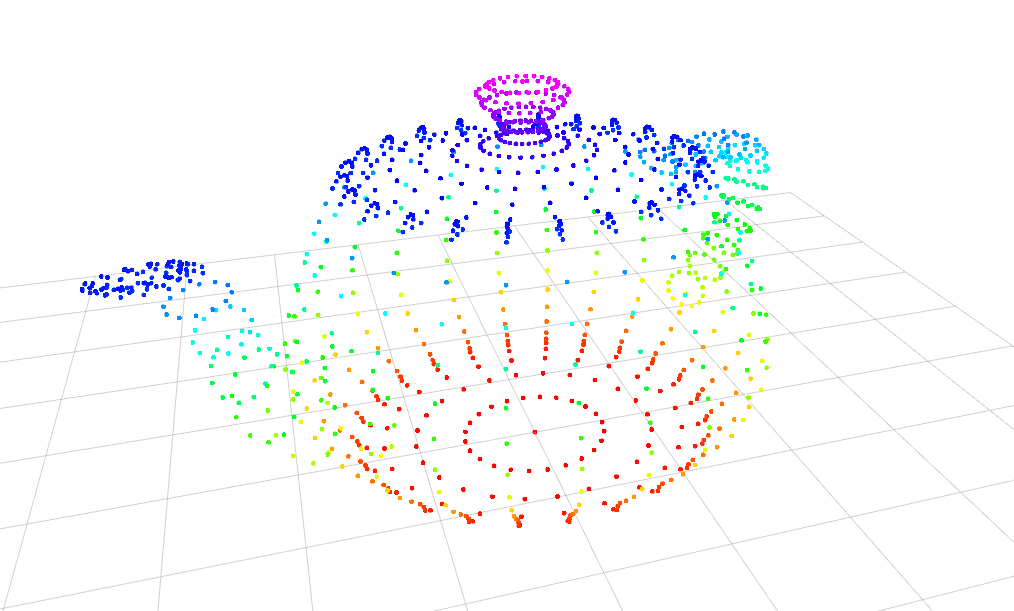
\includegraphics[width=0.50\textwidth]{headerimg}
    \caption{représentation d'un nuage de point dans l'espace}
    \label{fig:pointCloud1}
\end{figure}

Dans notre cas ici $P$ est un ensemble de points qui n'ont aucuns liens logique. En effet on considère l'ensemble des points comme non ordonné.
Mais notre vision actuelle est limité par rapport à ce qui est possible de faire avec un nuage de points. En effet rien ne nous empêche d'ajouter en plus des informations spatiale (les coordonnées) d'autres informations, tel que la couleur des points ou encore la direction de la normale associée (très utile pour le passage de nuages de points vers mesh 3D par la méthode de reconstruction de poisson que nous verrons plus tard). Dans ce cas le nuage de point obtenu est dit augmenté et on peut le représenter comme l'ensemble :

\[ P_{F} = \{ (x_{i}, f_{i}) | x_{i} \in \Re^{3}, f_{i} \in \Re^{D} \}_{i<N} \]

Ou $D$ est la dimension des informations liées à un point.
On utilise très souvent des nuages de points colorés (avec une information de dimension 3 : RGB) :

\begin{figure}[h]
    \centering
    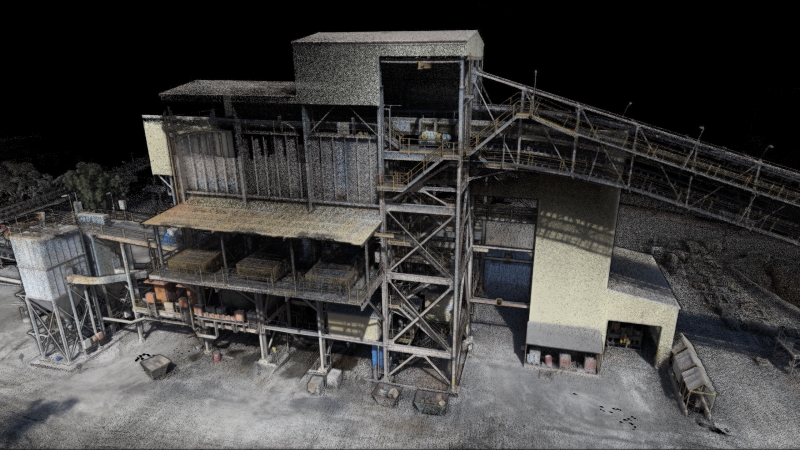
\includegraphics[width=0.50\textwidth]{ColoredPC}
    \caption{Nuage de point coloré}
    \label{fig:pointCloud2}
\end{figure}


En récapitulatif :

\begin{figure}[h]
    \subfloat[Espace vide]{
        \begin{minipage}[c][1\width]{
            0.3\textwidth}
            \centering
            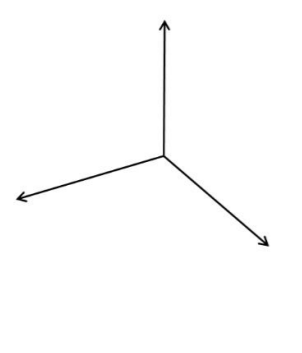
\includegraphics[width=1\textwidth]{Capture3}
        \end{minipage}}
    \hfill
    \subfloat[Ensemble $P$]{
        \begin{minipage}[c][1\width]{
            0.3\textwidth}
            \centering
            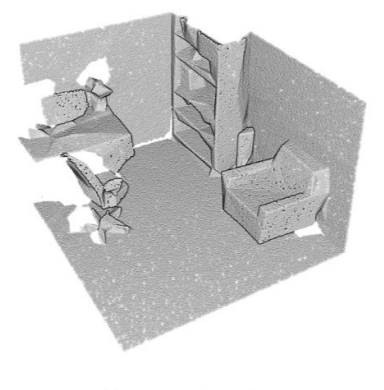
\includegraphics[width=1.1\textwidth]{Capture1}
        \end{minipage}}
    \hfill
    \subfloat[Ensemble $P_{F}$]{
        \begin{minipage}[c][1\width]{
            0.3\textwidth}
            \centering
            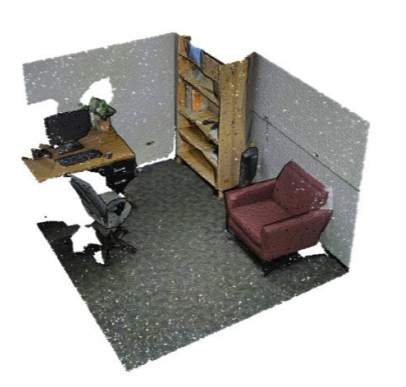
\includegraphics[width=1.2\textwidth]{capture2}
        \end{minipage}}
    \caption{}
    \label{fig:figure1}
\end{figure}

les nuages de points obtenus sont donc une représentation discrète et non ordonnée dans l'espace.

\FloatBarrier
\subsubsection{Maillages 3D}
\paragraph{•} Nous allons maintenant nous attarder sur la définition des maillages 3D ou mesh 3D.Un mesh 3D, de par sa plus grande complexité par rapport aux nuages de points, peut être défini de plusieurs façons. Nous allons ici nous attarder sur sa version la plus classique.
\paragraph{•} Un model 3D représente une collection de points (appelés vertex) dans l'espace connecté par des liens géométriques. On peut par exemple citer les liens sous forme de triangles, lignes ou surfaces.
Ce type de représentation permet donc à l'inverse des nuages de points d'avoir un ensemble de points ordonnés et donc liée les uns avec les autres pour former une forme géométrique. Il est alors possible d'en extraire des informations plus riche que les nuages de points. On peut par exemple obtenir la surface du modèle ou encore son orientation.



\begin{figure}[h]
    \centering
    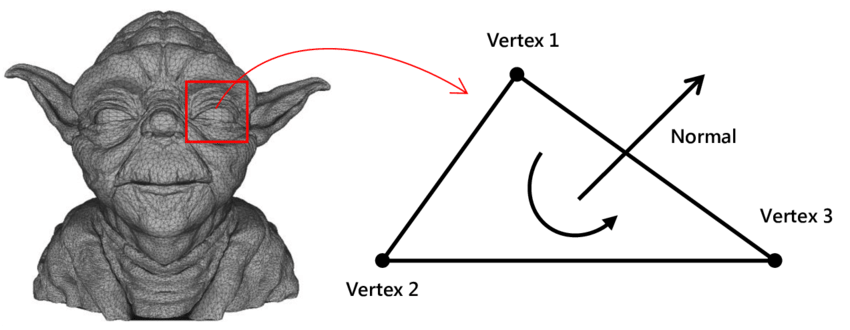
\includegraphics[width=0.50\textwidth]{Structure-of-a-3D-triangle-mesh}
    \caption{Exemple de mesh 3D}
    \label{fig:Structure-of-a-3D-triangle-mesh}
\end{figure}



On ne pas donner de définition mathématique des modèles 3D (possible mais sort du contexte de ce rapport). En effet pour avoir une définition exacte il faut préciser le cadre : mesh structuré,structuré par blocs ou non structuré.
Nous nous contenteront donc ici d'une approche plus générale.

Les nuages de points peuvent être vu comme une vision discrète non ordonnée du monde 3D alors que les modèles 3D nous donne une vison continue ordonnée, plus riche.
\FloatBarrier


%%%%%%%%%%%%%%%%%%%%%%%%%%%%%%%%%%%%%%%%%%%%%%%%%%%%%%%%%%%%%
%% METHODES D'ACQUISITION
%%%%%%%%%%%%%%%%%%%%%%%%%%%%%%%%%%%%%%%%%%%%%%%%%%%%%%%%%%%%%
\section{Méthodes d'acquisition}
Il est maintenant question d'étudier les différentes façons dont il est possible d'obtenir une représentation 3D du monde réel sous forme de nuages de points ou de mesh 3D. Nous allons pour faire présenter 3 catégorie de méthodes différentes. Une première catégorie qui permet l'acquisition de nuages de points (scanner laser), une seconde catégorie permettant d'obtenir des volumes 3D sous forme de mesh (caméra avec vison de profondeur, IRM...) et finalement des méthodes dites hybrides qui permettent l'obtention de mesh et de nuages de points (photogrammétrie, stéréographie...).

%% Mettre cette étape en conclusion
Il est important de noter que l'obtention de mesh 3D est très difficile car de demande lecture continue de l'espace 3D, cela est souvent uniquement possible en espace restreint et limité en temps. De l'autre coté l'obtention de nuages de points est beaucoup plus simple et permet une reconstruction du mesh 3D. C'est souvent la méthode que l'on utilise. Beaucoup plus simple à mettre en place.
\subsection{Acquisition des nuages de points}
\subsubsection{Principe}
\paragraph{•} La méthode d'acquisition la plus représentative lorsque l'on parle de nuages de points et la plus répendue aujourd'hui est celle dite des scanneur laser. Dans ce cadre les LiDAR (Light Detection And Ranging) sont les capteurs les plus privilégiées. Bien que les LiDAR peuvent être fondés sur différentes technologies, le principe reste identique : il s'agit d'un "Radar électromagnétique", un émetteur qui émet une pulsation électromagnétique qui se réfléchie sur un sujet pour ensuite être captée par un récepteur. La durée entre l'émission et la réception de l'impulsion permet de déterminer la distance à l'objet.

\begin{figure}[h]
    \centering
    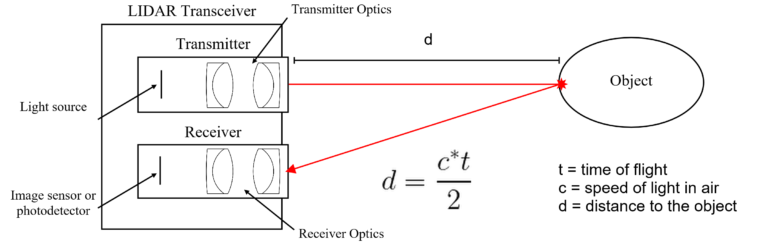
\includegraphics[width=0.50\textwidth]{lidarWorks}
    \caption{Schéma de fonctionnement d'un LiDAR}
    \label{fig:lidarWork}
\end{figure}
\FloatBarrier
Cette méthode permet alors d'obtenir des nuages de points de très grande qualité, ci-dessous quelques exemples :

\begin{figure}[h]
    \centering
    \subfloat[ Vue dans l'axe du LiDAR]{{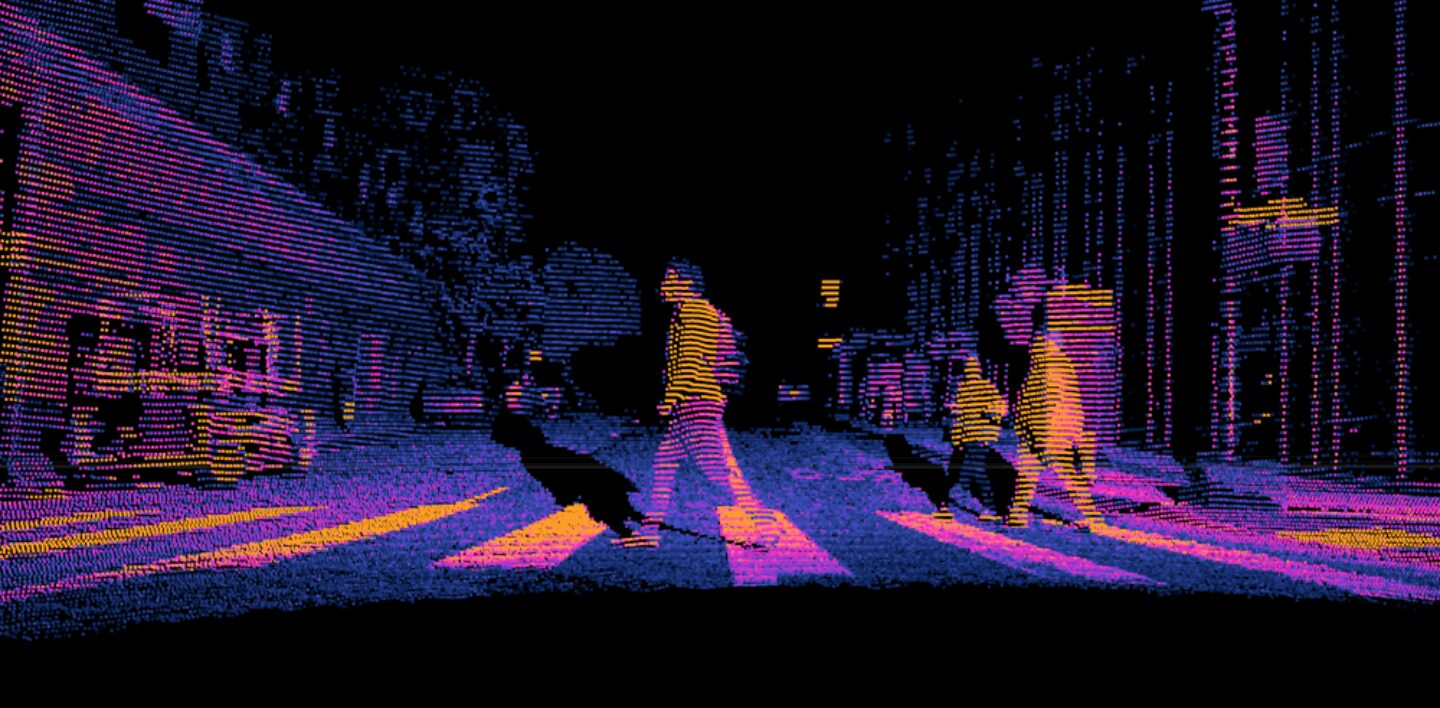
\includegraphics[width=6cm]{FrontViewLIdar} }}
    \qquad
    \subfloat[ Vue globale de la carte 3D]{{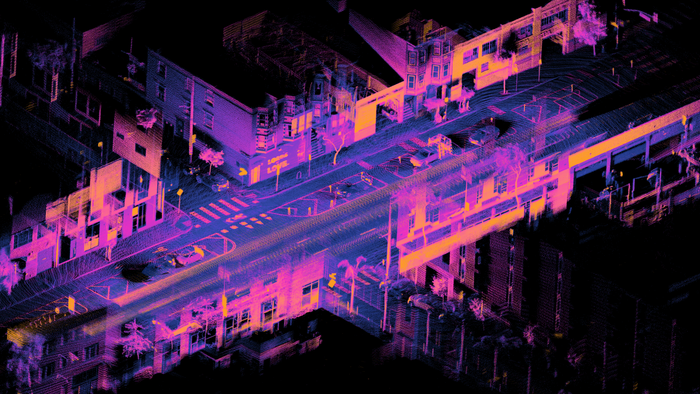
\includegraphics[width=5cm]{lidarExamplePC} }}
    \caption{Nuages de points obtenus d'un LiDAR Ouster OS1-128}
    \label{fig:PCLidar}
\end{figure}
\FloatBarrier

Nous verrons dans la suite comment ces nuages de points peuvent être traités pour permettre la génération de maillage 3D. La même méthode peut être appliquer ici pour permettre l'obtention de maillage 3D à partir des données LiDAR.

\subsubsection{capteurs}
Le LiDAR nécessite des équipements spécifiques et couteux. Cependant, leur cout de production diminue avec la democratisation de la technologie (integration de scanner LiDAR dans plusieurs flagship smartphones).
\begin{figure}[h]
    \centering
    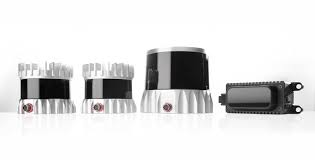
\includegraphics[width=0.50\textwidth]{ousterLidars}
    \caption{Gamme de capteur LiDAR Ouster}
    \label{fig:ousterLidars}
\end{figure}
\FloatBarrier


\subsection{Acquisition maillages 3D}
\subsubsection{Principe}
\paragraph{•} En pratique l'acquisition des maillages 3D est beaucoup plus complexe que celle des nuages de points. En effet les maillages 3D comportent une information continue et précise de la géométrie 3D, une représentation exacte de la surface du modèle. Or être capable de précisément déterminer le volume et la surface de l’environnement réel demande des technologies très complexes.
On peut néanmoins citer certaines de ces technologies et leurs limitations. On a notamment les scanners IRM qui permettent d'obtenir une information volumétrique (à partir de plusieurs tranches misent bout à bout et interpolés) mais ne sont opérationnel que sur de petits volumes.
\newline
D'autre part avec l’apparition de méthodes plus modernes, qui utilisent l'intelligence artificielle on peut aujourd’hui reconstruire un modèle 3D à partir d'une simple information 2D. Nous allons nous attarder ici à l'état de l'art actuel, pifuhd développé par facebook reasearch lab \cite{saito2020pifuhd}.
La solution proposé permet de générer un mesh 3D à partir d'une image 2D d'une personne.

\begin{figure}[h]
    \centering
    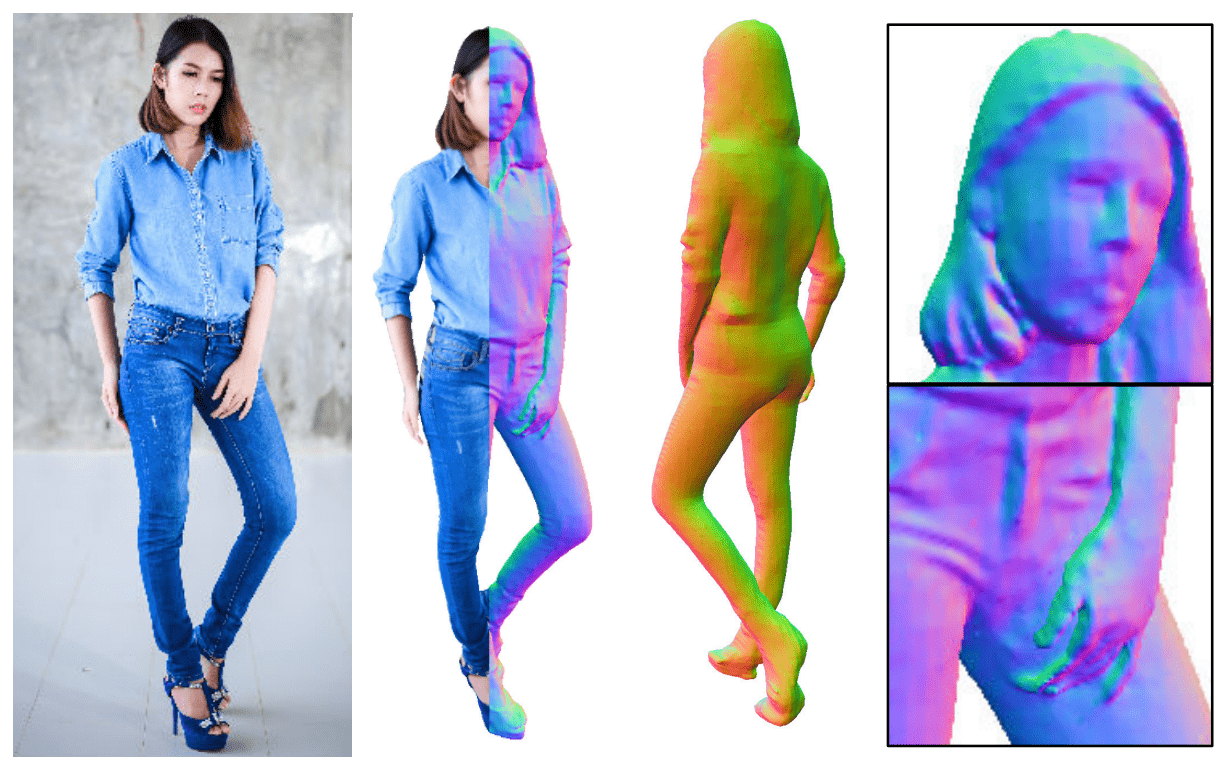
\includegraphics[width=0.50\textwidth]{pifuhd}
    \caption{Etapes de génération de pifuhd}
    \label{fig:pifuhd}
\end{figure}
\FloatBarrier

Le logiciel utilise une méthode d'optimisation implicite à partir d'une analyse de l'image 2D à plusieurs niveaux (Multi-Level Pixel-Aligned Implicit Function optimization). On peut se représenter cette méthode comme une méthode des templates. En effet tout est ici, comme ci nous partions d'un model 3D universel représentant une personne et on va le déformer pour qu'il corresponde aux proportions de l'image.

\begin{figure}[h]
    \centering
    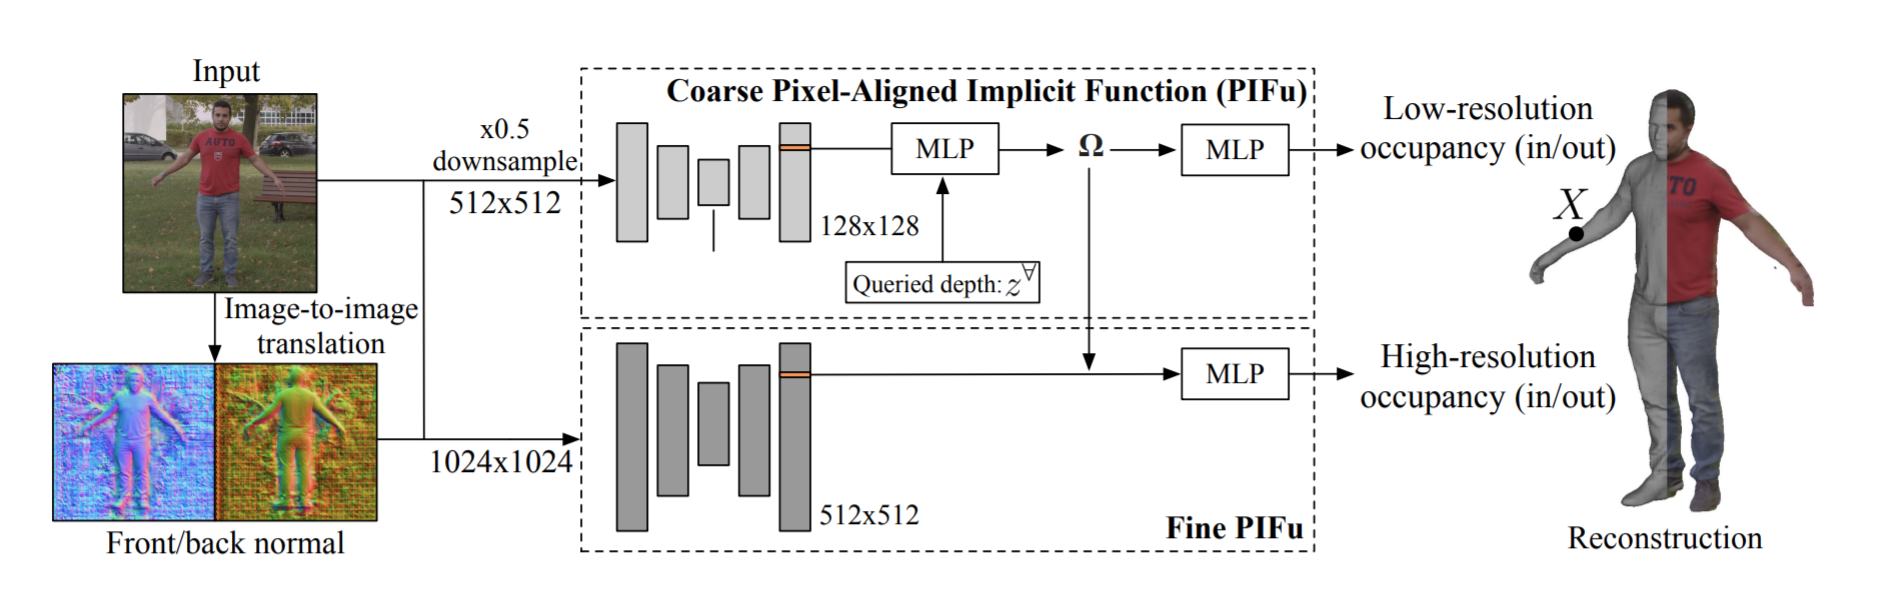
\includegraphics[width=0.8\textwidth]{pifuhdWork}
    \caption{Fonctionnement interne de pifuhd}
    \label{fig:pifuhdWork}
\end{figure}
\FloatBarrier

Ces méthodes de génération de modèles 3D à partir d'une information de dimension inférieure (ie. image 2D) est voué à être de plus en plus utilisé, en effet elle permet l'obtention d'un model 3D de meilleure qualité et avec une complexité moindre qu'en passant par la génération d'un nuage de point. Ce genre de méthode, bien qu'ici réduite à la simple modélisation de personnes, à été aussi étendue à d'autre domaines, comme l'imagerie médicale ou la génération de surface topographiques (DSM : Digital elevation terrains)\cite{DSM}.


\subsection{Méthodes hybrides}

\paragraph{•} Pour le moment nous avons vu comment obtenir des nuages de points et des maillages 3D directement et indépendamment l'un de l'autre. Mais dans la pratiques il n'est pas rare de passer par des méthodes hybrides ou l'on génère en premier lieu un nuage de point, puis c'est à partir de ce nuage de point que l'on génère le maillage 3D avec différentes méthodes de reconstruction. Il existent deux méthodes très largement utilisées :

\subsubsection{Photogrammétrie} La photogrammétrie  consiste a utiliser des collections de prises de vue 2D d'un sujet pour en recréer une représentation tridimensionnelle. La photogramétrie se fait en trois grandes étapes. il faut d'abord positioner les photos prises dans l'espace afin d'obtenir les position et orientation du capteur lors de la prise, on appelle cette étape bundle adjustment. Puis vient l'étape de projection d'un ensemble de point (appelé features) dans l'espace. C'est avec cette ensemble de ces points projetés que l'on peut finalement densifier le nuage de point ainsi obtenu. Ces méthodes sont appelées sfm (structure from motion) \cite{orb} \cite{mvg} :

\begin{figure}[h]
    \centering
    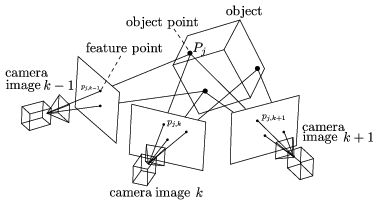
\includegraphics[width=0.5\textwidth]{sfm}
    \caption{Structure From Motion}
    \label{fig:sfm}
\end{figure}
\FloatBarrier

On peut alors obtenir sous forme d'un nuage de point dense la représentation de l'environnement :

\begin{figure}[h]
    \centering
    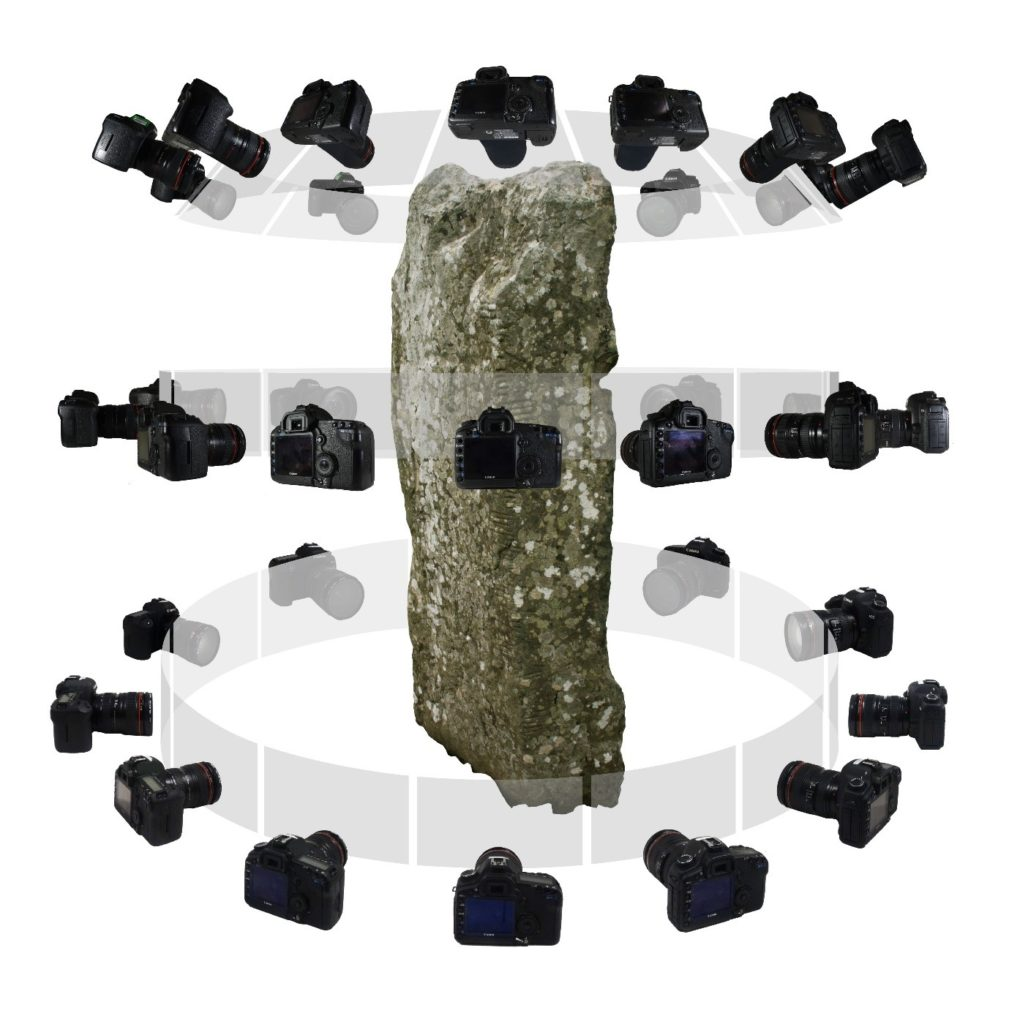
\includegraphics[width=0.3\textwidth]{photog}
    \caption{Nuage de point reconstruit à partir des images}
    \label{fig:photog}
\end{figure}
\FloatBarrier


Il est alors possible à partir de ce nuage de point d'obtenir un maillage 3D. Il existe plusieurs méthodes le permettant. La plus connue est celle dite de reconstruction de poisson \cite{poisson}, mais elle demande la connaissance des normale associée à chaque point (ce qui rajoute une étape de calcul). Nous allons donc ici présenter une méthode plus générale : Advancing Front Surface Reconstruction \cite{dddddd}. En effet cette méthode avec un peu de pré traitement et de post traitement permet l'obtention d'un maillage 3D de très bonne qualité à partir d'un nuage de point dense.

\begin{figure}[h]
    \centering
    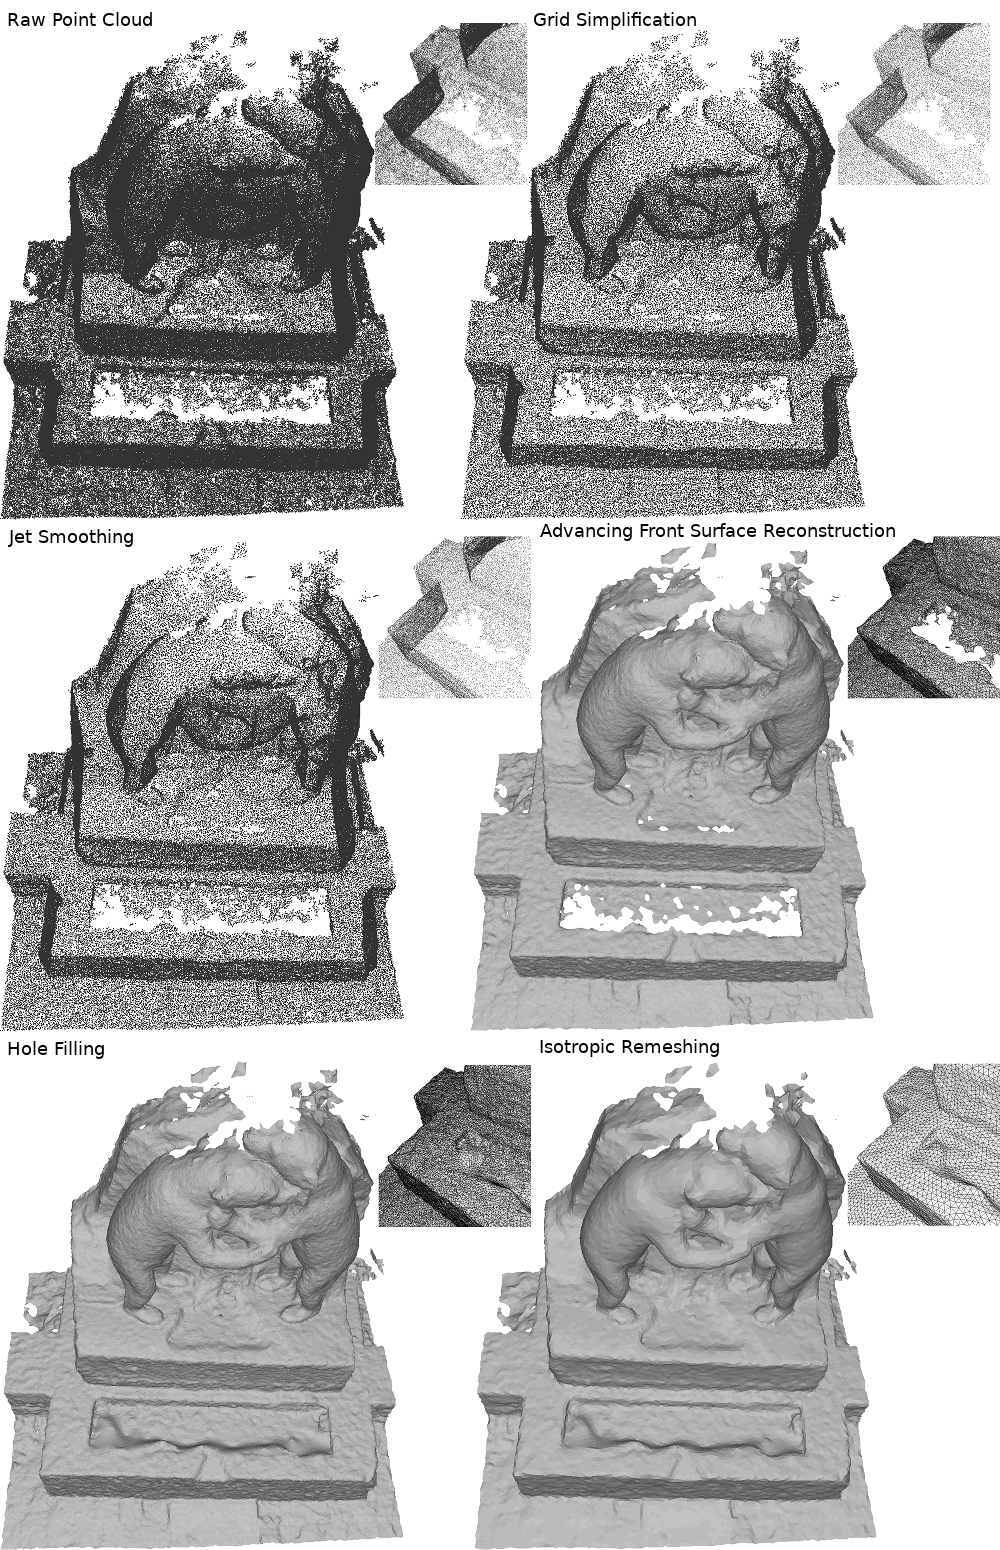
\includegraphics[width=0.4\textwidth]{reconstruction}
    \caption{Exemple de reconstruction utilisant cette méthode à l'aide de CGAL}
    \label{fig:photog}
\end{figure}
\FloatBarrier


\subsubsection{Depth map} 
Finalement nous pouvons présenter les cameras à profondeur de champ (depth cameras). Elle ne permettent pas directement d'obtenir un mesh 3D, mais elle fournissent une surface pouvant être utilisé pour la reconstruction du mesh 3D. Similaire à la photogrammétrie, elles sont constitué de deux cameras qui permettent d'obtenir une vision stéréo, on peut alors extraire une information de profondeur sous forme de nuage de point puis d'image 2D associant à chaque pixel sa profondeur relative par rapport au capteur qui peut être utilisé par la suite pour générer un mesh 3D de la surface situé en face de la caméra (Stéréoscopie) \cite{book1} .

\begin{figure}[h]
    \centering
    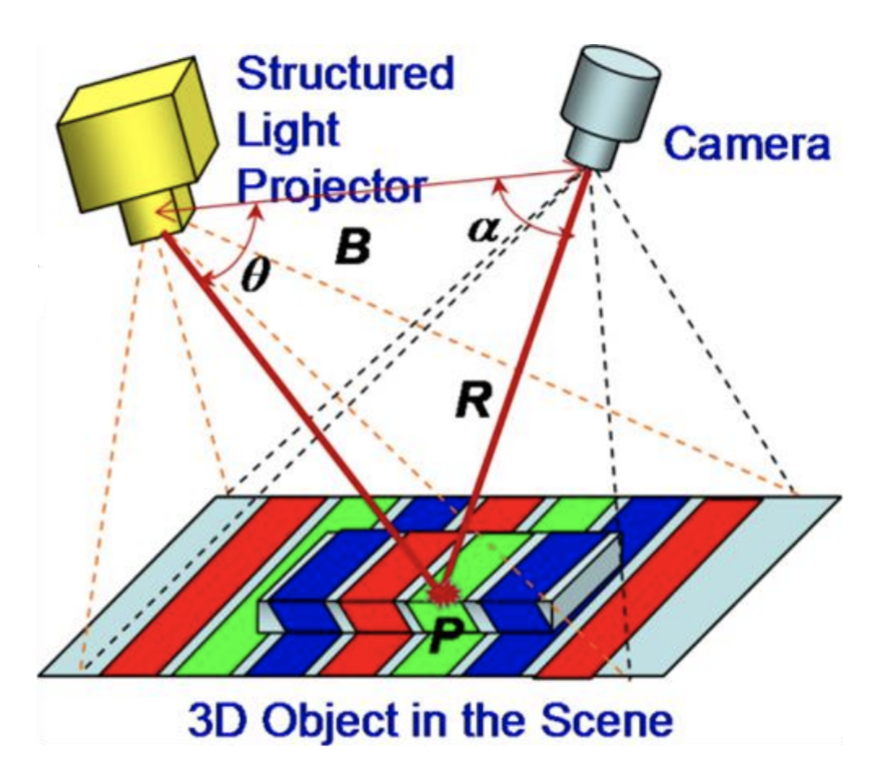
\includegraphics[width=0.4\textwidth]{stt}
    \caption{Fonctionnement de la Stéréoscopie}
    \label{fig:pifuhdWork2}
\end{figure}
\FloatBarrier

On obtient alors une carte de la profondeur vu par la caméra (depth map) :

\begin{figure}[h]
    \centering
    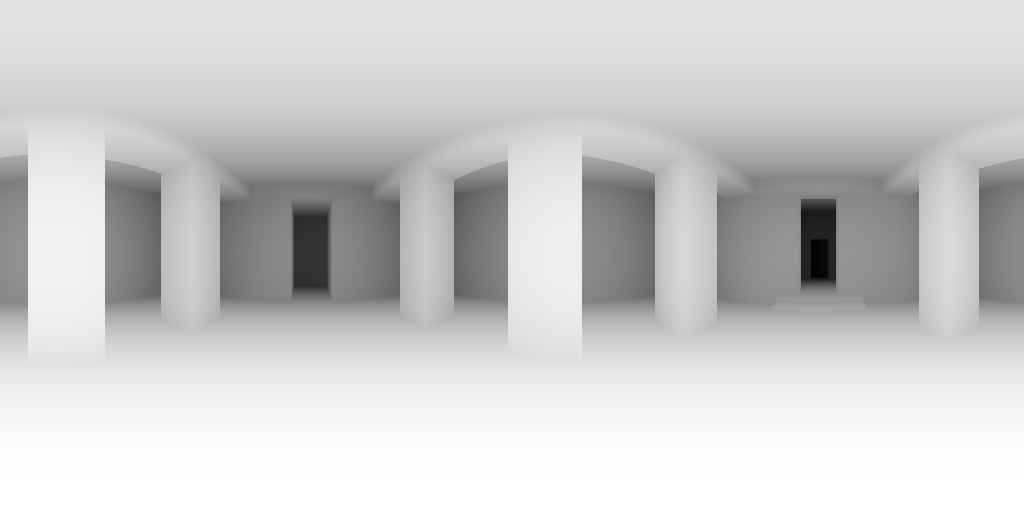
\includegraphics[width=0.8\textwidth]{depthmap}
    \caption{image obtenue, noir = loin, blanc = près}
    \label{fig:pifuhdWork3}
\end{figure}
\FloatBarrier

Pour obtenir un modèle 3D fermé représentatif, il faut alors se déplacer autour de l'objet pour le scanner. En pratique le processus est plus complexe que cela, il faut utiliser une carte globale et enregistrer chaque image 2.5D (depth map), un framework tel que supereight \cite{super} permet de réaliser ce genre de carte 3D.
On récupère alors l'environnement sous forme de mesh 3D :

\begin{figure}[h]
    \centering
    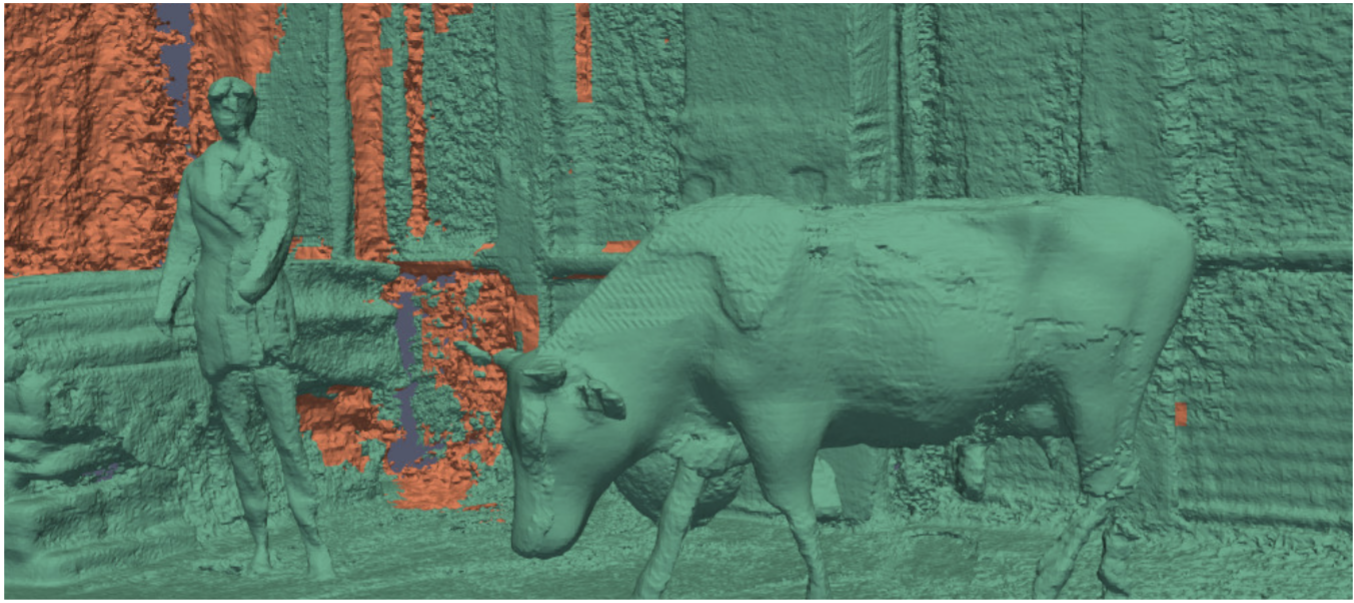
\includegraphics[width=0.8\textwidth]{super}
    \caption{Modèle 3D de l'environnement obtenu}
    \label{fig:super}
\end{figure}
\FloatBarrier


\subsection{Conclusion}


\subsubsection{précision}
\paragraph{•} Le LiDAR permet une très grande précision qui peut même être amélioré avec l'utilisation et la modulation des longueurs d'ondes. Cependant, cette précision est étroitement liée a la nature de l'objet. En effet, les objets foncés réfléchissant moins les ondes électromagnetic, les niveaux de bruits sont plus elevés. De la meme maniere, en fonction de la longueur d'onde, les sujets transparents ou à effet miroirs rendent donc la modélisation pratiquement impossible.
Dans le cas de la photogrammétrie, la précision est encore plus susceptible de varier. En effet, en fonction du type d'utilisation (de la photographie aérienne aux sujets d'échelle humaine) la résolution varie. En effet, comme cette méthode repose sur l'analyse de photographies, l'algorithme de traitement ainsi que la qualité des photos influencent grandement le résulta final. De plus, on retrouve les mêmes problèmes qu'avec le LiDAR c'est-à-dire avec les faibles contrastes et objets transparents.

%%%%%%%%%%%%%%%%%%%%%%%%%%%%%%%%%%%%%%%%%%%%%%%%%%%%%%%%%%%%%
%% METHODES DE STOCKAGE
%%%%%%%%%%%%%%%%%%%%%%%%%%%%%%%%%%%%%%%%%%%%%%%%%%%%%%%%%%%%%
\section{Méthodes de stockage}
%%%%%%%%%%%%%%%%%%%%%%%%%%%%%%%%%%%%%%%%%%%%%%%%%%%%%%%%%%%%%
%% DOMAINES D'APPLICATION
%%%%%%%%%%%%%%%%%%%%%%%%%%%%%%%%%%%%%%%%%%%%%%%%%%%%%%%%%%%%%
\section{Domaines d'applications et utilisation}
\paragraph{•} Les mesh permettent donc un rendu surfacique sur laquelle s'applique une texture alors que les nuages de points est une liste de points finie et non ordonnée.
En pratique, les nuages de points sont utilisés principalement dans la reconnaissance 3D d'objets, par exemple dans le cadre des systèmes embarqués ou de la robotique. Bien que les nuages de points peuvent être utilisés, on utilise généralement les maillages de points pour créer des modèles CAO 3D de pièces mécanique, pour les modèles météorologiques ou dans le contrôle de qualité. Les mesh sont particulièrement utilisés grâce à leurs caractères surfaciques pour les applications de visualisation, d'animation, de rendu et de personnalisation de masse.

\section{conclusion}
\paragraph{•} Ne pas oublie de parler du cout de chaque méthode

\chapter{Etude de cas : Les Smart Cities}



%%%%%%%%%%%%%%%%%%%%%%%%%%%%%%%%%%%%%%%%%%%%%%%%%%%%%%%%%%%%%
%% 
%%%%%%%%%%%%%%%%%%%%%%%%%%%%%%%%%%%%%%%%%%%%%%%%%%%%%%%%%%%%%
\section{Introduction}
Le concept de Smart City est fondé sur les intérêts qu'auraient les métropoles à utiliser les technologies d'information et de communication pour y booster l'efficacité des différents flux et minimiser les pollutions. En effet, l'objectif est de remplacer les prises de décision politiques par des choix basés sur des masses de données récoltées par un grand nombre de capteurs situés partout dans la ville. Cela nécessite l'utilisation d'un modèle 3D poussé : les informations obtenues en temps réel par les capteurs ne prennent un sens que lorsqu'ils sont mis en relation et en contexte. En outre, certaines études ne peuvent en pratique se faire qu'avec un modele 3D. Par exemple l'étude des écoulement et drainage des eaux.

%A faire : 
%- Introduire ce qu'est une smart city et comment ça peut être l'évolution de notre mode dans les prochaines années

%\section{Les enjeux}
%- parler de l'enjeu d'avoir une représentation 3D précise de celles ci (aller voir sur internet, exemples : calcul des flux pour l'optimisation, gestion thermique, gestion des risques (criminels  -> camera), réseau centralisé des risques...)
%- Expliquer que c'est un domaine d'avenir : mettre des budgets allouer ou des papier sur là ou on va
%
% * <anatole.maurer@telecom-sudparis.eu> 22:42:07 10 Feb 2022 UTC+0100:
% du coup tout ca c'est deja un peu dans lintro ...
%Lisez ce papier https://www.gim-international.com/magazines/gim-international-september-october-2018.pdf vous verez toute les Utilisation possibles.


\section{Modélisation 3D}

La première étape pour obtenir une version jumelle d'une ville dans le monde 3D est d'obtenir sa copie. En effet, il nous en faut une représentation 3D. Cependant, il est nécessaire d'avoir une représentation particulière : il nous faut une représentation qui puisse être ensuite utilisée de façon complexe. Il nous faut donc une version enrichie de la ville, une version qui ne soit pas juste de la donnée géométrique mais qui puisse contenir les interactions de chaque composant les uns avec les autres (par exemple les feux de circulation avec la gestion de flux...)
Nous allons étudier comment obtenir cette représentation 3D en plusieurs étapes : il faut tout d'abord en obtenir une version 3D sous forme de nuage de points, puis la convertir en mesh, avant d'intégrer cette vision dans un moteur de calcul et si possible de rendu graphique.

\subsection{Acquisition 3D}
Ce rapport portant sur la notion de nuages de points et de maillages 3D, nous avons pu précédemment expliciter les différences et les liens entre ces deux représentations de données 3D. La reconstruction dans le monde virtuel d'une ville passe donc en premier lieu par une acquisition sous forme de nuage de points denses à plusieurs niveaux des données géométriques de la ville. En effet, comme nous avons pu le voir, les relevés laser permettent une acquisition simple des nuages de points et avec une grande précision sur de longues distances.
Dans la plupart des cas, la collecte est faite à deux échelles : des scanners terrestre et aérien sont utilisés. De même une combinaison de méthodes devra être utilisée; dans notre cas le plus souvent on retrouve la photogrammétrie et les scanners LiDAR.

\subsubsection{Scan au niveau du sol}
La collecte des données 3D au niveau du sol se fait très souvent à l'aide de scanner LiDAR, leur grande précision et  leur capacité de scanner rapidedement permet une plus grande flexibilité. Pour ce faire il est nécessaire d'utiliser des algorithmes de SLAM (Simultaneous Localisation And Mapping) \cite{LOAM} qui permettent de suivre le capteur et de projeter les nuages de points obtenus dans une carte 3D globale qui peut ensuite être combinée avec d'autres cartes pour obtenir la ville :

Pour ce faire il nous faut un rig avec un LiDAR et des cameras RVB pour obtenir un nuage de points colorés :
\begin{figure}[h]
    \centering
    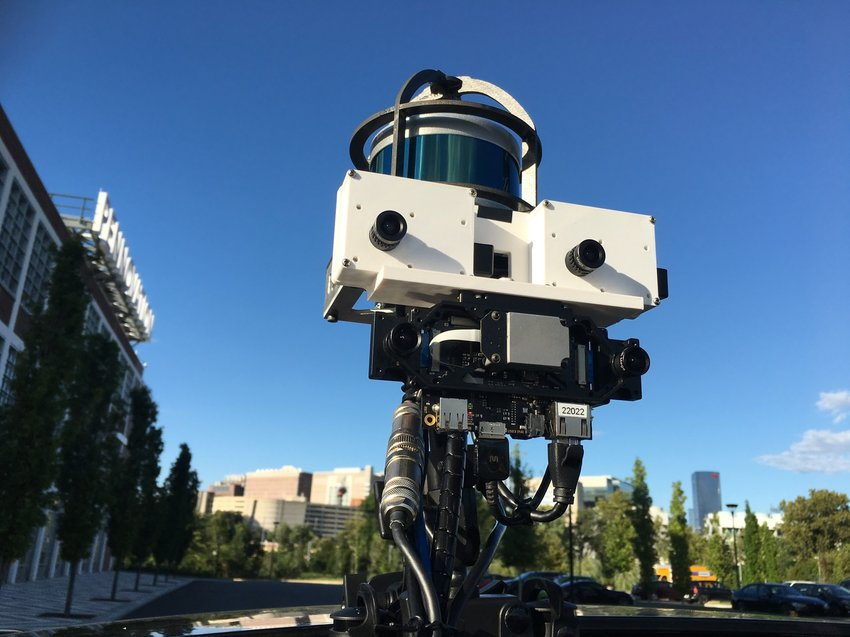
\includegraphics[width=0.50\textwidth]{rig}
    \caption{Exemple de rig de scan au sol}
    \label{fig:solrig}
\end{figure}
\FloatBarrier

Puis l'utilisation d'un algorithme de SLAM pour enregistrer le nuage de points. On peut alors, pour obtenir une carte avec une position absolue, combiner des données GPS et inertielles dans le SLAM directement :

\begin{figure}[h]
    \centering
    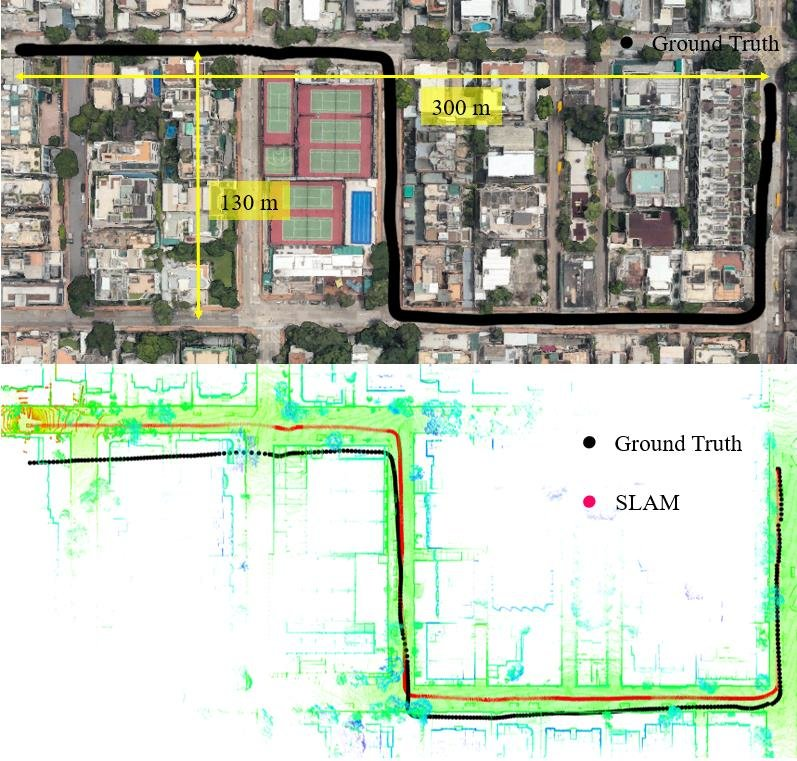
\includegraphics[width=0.50\textwidth]{slam}
    \caption{Chemin du capteur retrouvé par l'algo de SLAM}
    \label{fig:solrig}
\end{figure}
\FloatBarrier

\newpage

Finalement après avoir scanné la ville, on obtient un nuage de points au niveau du sol précis de celle ci :
\begin{figure}[h]
    \centering
    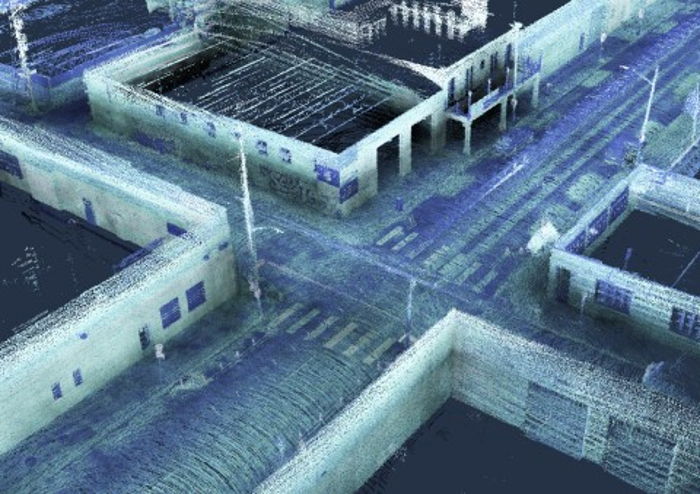
\includegraphics[width=0.50\textwidth]{ground}
    \caption{Vision en nuage de points au niveau du sol}
    \label{fig:sol}
\end{figure}
\FloatBarrier

\subsubsection{Cartographie 3D aérienne}

Il faut maintenant obtenir une vue plus globale de la ville pour, une fois combinée avec notre scan au sol, obtenir l'ensmeblede la ville.
Pour ce faire nous allons combiner les méthodes de photogrammétrie et de scan laser à bord d'un avion : le scan laser permet d'avoir avec précision les distance, tandis que le scan photogrammétrique permet d'avoir  la couleur associée ainsi que certains détails.
\begin{figure}[h]
    \centering
    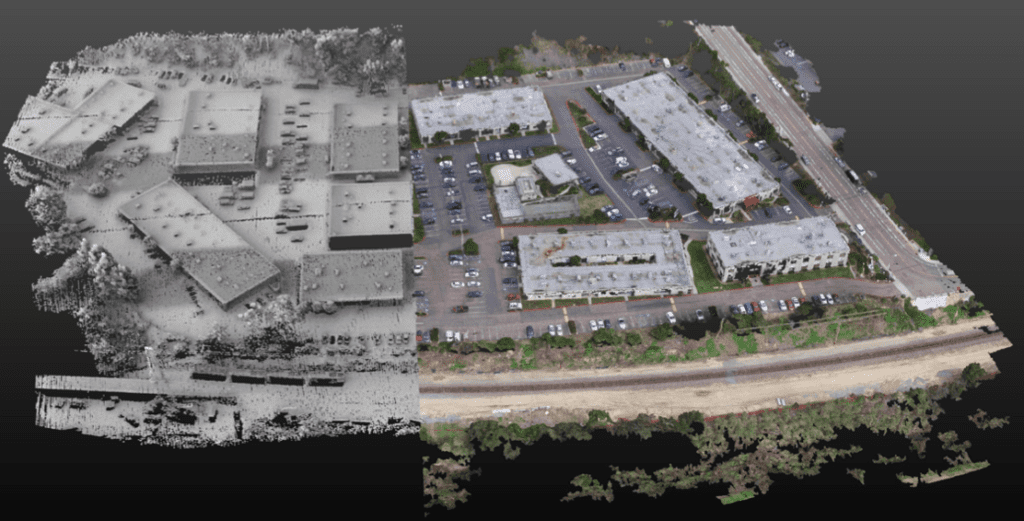
\includegraphics[width=0.8\textwidth]{lidarPhoto}
    \caption{Fusion des données LiDAR et Photogrammétriques}
    \label{fig:sol}
\end{figure}
\FloatBarrier

\newpage

Une fois ces deux types d'acquisitions terminées, il faut ensuite combiner les nuages de points obtenus pour récupérer une carte de nuage de points dense.
\newline

\begin{figure}[h]
    \centering
    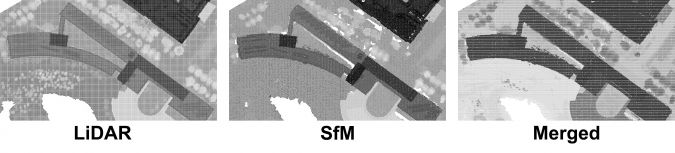
\includegraphics[width=0.8\textwidth]{merge}
    \caption{Combinaison des deux cartes : sol + aérien}
    \label{fig:sol}
\end{figure}
\FloatBarrier
C'est à partir de ce nuage de points dense que nous travaillerons dans la suite.
\begin{figure}[h]
    \centering
    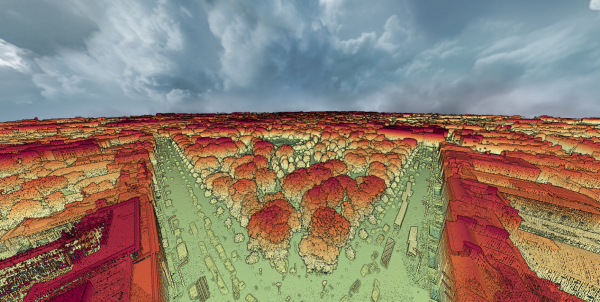
\includegraphics[width=0.8\textwidth]{cityscan}
    \caption{Résultat final de la ville en nuage de points}
    \label{fig:sol}
\end{figure}
\FloatBarrier

\paragraph{Pour aller plus loin} Nous n'avons ici fait que présenter la surface du sujet. Cependant, il y a beaucoup de recherche dans ce domaine; Que ce soit au niveau du SLAM : comment arriver à faire des slam de très grande envergure en limitant l'erreur \cite{slamLargeScale} ou comment réaliser des slam avec différents types de données (GPS, IMU...), mais aussi sur de la photogrammétrie de grandes étendues \cite{LargeScale}. Tout comme la gestion des nuages de points, la fusion de nuages denses est un champ actif de recherche. Cependant, la présentation de tous ces domaines sortirait du cadre de ce document.

\subsection{Transformation en maillage 3D et format spécialisé}

Une fois le nuage de points obtenu, il est maintenant question de le transformer en maillages 3D qui, si possible, pourront être utilisés par la suite dans une application spécialisée pour associer à chaque catégorie d'intérêt un traitement spécifique : centrale électrique, résidences, immeubles...
\newline
Pour réaliser cette différenciation nous allons devoir classifier le nuage de points. La recherche dans ce domaine est la aussi très dynamique. Pour ce faire, des méthodes de classification algorithmique seront généralement utilisées : Support Vector Machine, K nearest search ou random forest. Cependant, les méthodes par machine learning deviennent de plus en plus concluantes. On peut par exemple citer : kpconv net \cite{thomas2019KPConv} ou encore pointnet++ \cite{qi2017pointnet}.
\newline
Grâce à ces différentes méthodes, on peut alors segmenter notre nuage de points :
\begin{figure}[h]
    \centering
    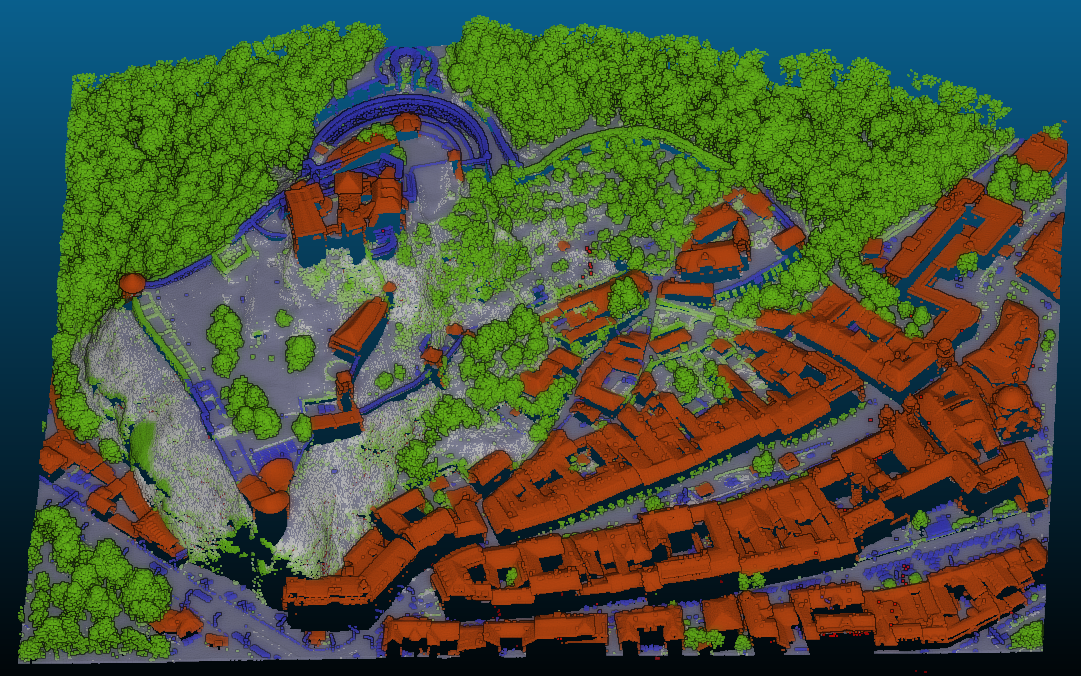
\includegraphics[width=0.65\textwidth]{clas}
    \caption{Nuages de points classifiés}
    \label{fig:sol}
\end{figure}
\FloatBarrier

A partir de ce nuage classifié, il vient alors la reconstruction de modèle sous forme de maillage 3D. Ici aussi, en fonction du type de donnée que l'on veut récupérer à la fin la reconstruction ne sera pas la même. Par exemple les bâtiment devront être convertis sous le format de données BIM (Building information modeling), le sol sous forme DST (Digital Surface Terrain), etc. Cette étape sera ici considérée comme une étape de conversion du nuage de points en maillages 3D. En effet, comme nous l'avons vu précédemment, pour permettre un rendu visuel optimisé, pour le traitement et l'analyse de ces données, l'utilisation de maillages 3D est nécessaire (impossible d'obtenir des résultats concluant sous forme de nuages de points).
Nous obtenons alors un modèle 3D sous forme de maillages 3D très précis de la ville :

\begin{figure}[h]
    \centering
    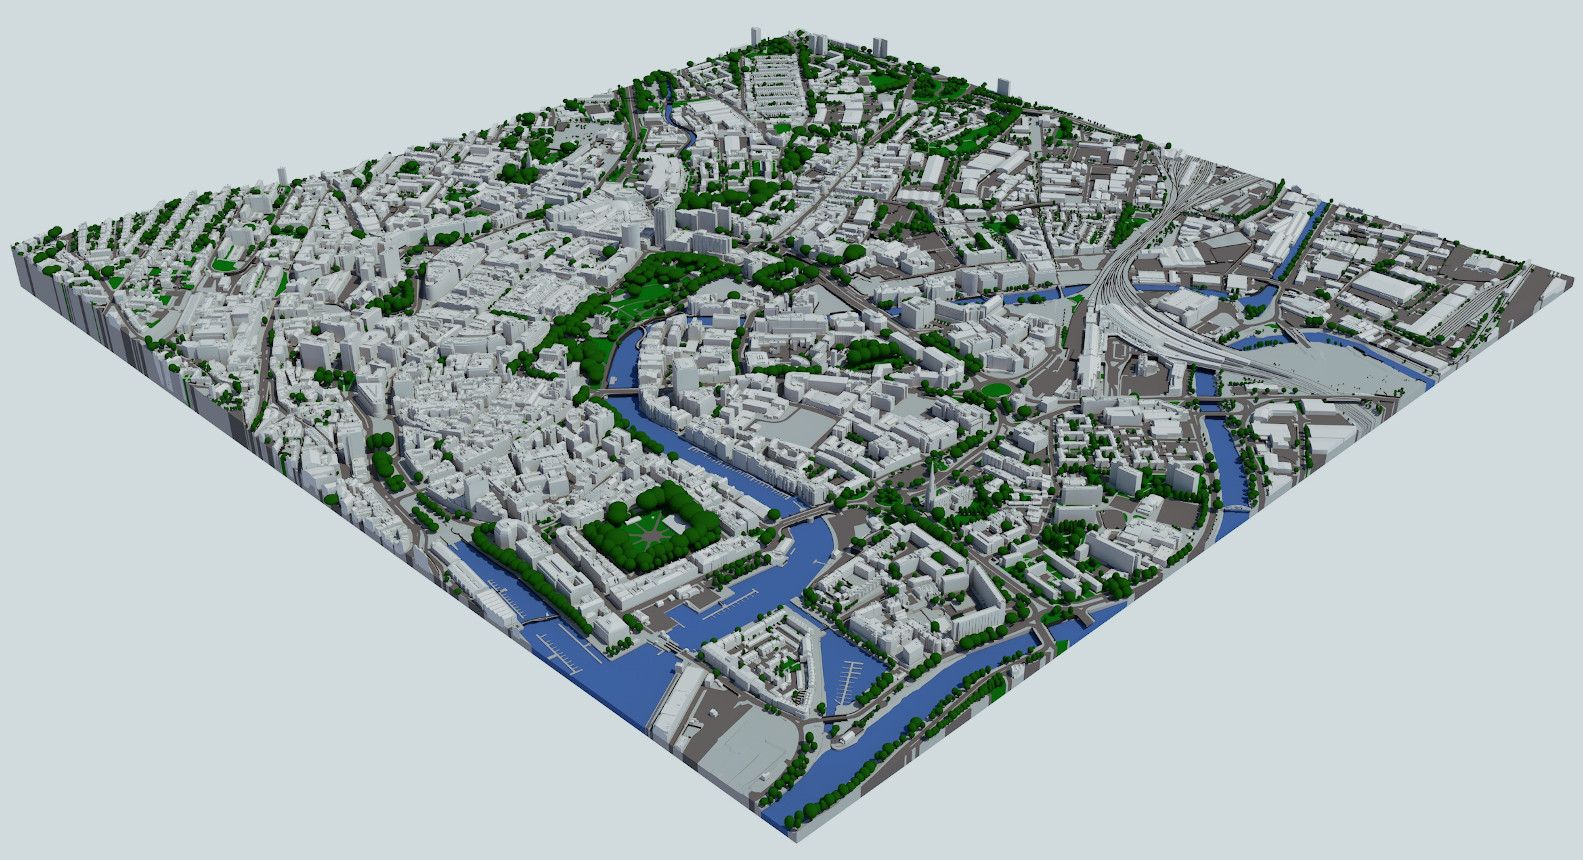
\includegraphics[width=0.65\textwidth]{globalmap}
    \caption{Jumelle virtuelle de notre ville}
    \label{fig:sol}
\end{figure}
\FloatBarrier

\section{Utilisation de la donnée 3D}

Une fois les données traitées et la ville virtuelle jumelle obtenue, nous pouvons maintenant l'utiliser pour visualiser, analyser ou simuler ses états : nous avons construit une représentation globale de la ville.

\subsection{Simulation}
La ville jumelle obtenue peut être utilisée dans le cadre de simulation grandeur nature avec une très grande complexité. Aujourd'hui les besoins de simulation sont de plus en plus grands : simulation des flux de personnes, des flux d'air sur les bâtiments, de l'eau, des voitures... Tout ceci est permis de par le fait que la ville virtuelle jumelle est une copie presque parfaite. De même pour le monitoring en temps réel : cette copie virtuelle peut être utilisée.

\begin{figure}[h]
    \centering
    \subfloat[ Simulation des flux d'air]{{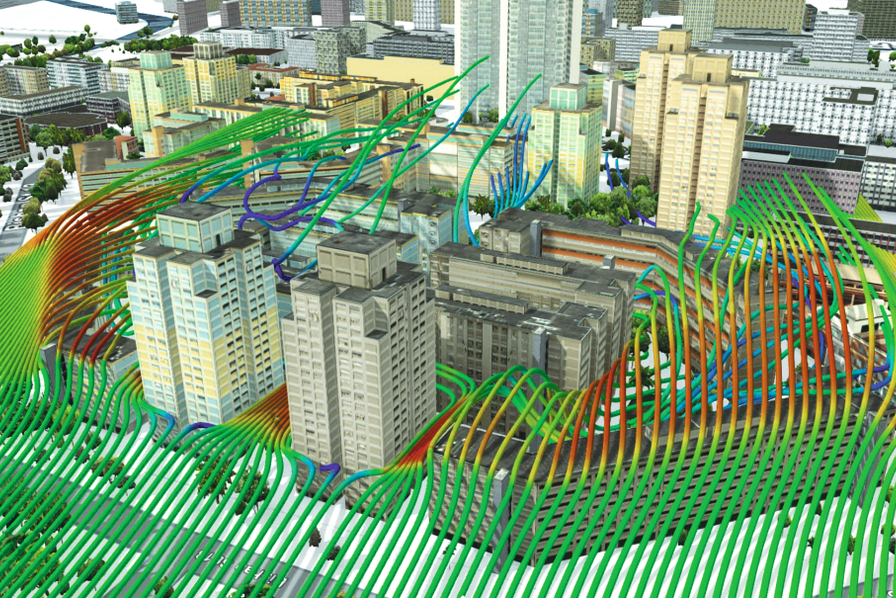
\includegraphics[width=7cm]{simmm} }}
    \qquad
    \subfloat[ Simulation de pertes thermiques]{{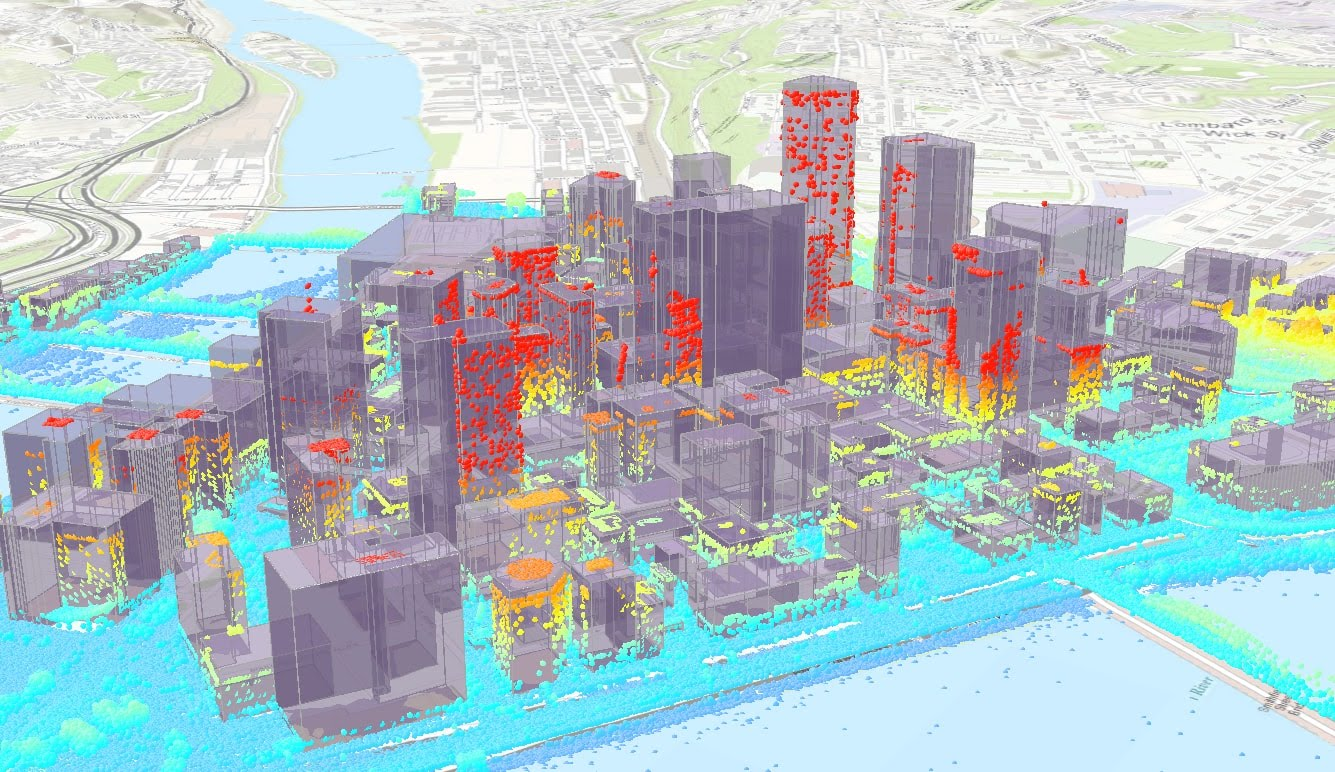
\includegraphics[width=7cm]{sim2} }}
    \caption{Utilisation de la copie virtuelle pour la simulation}
    \label{fig:Ud}
\end{figure}
\FloatBarrier


\subsection{Visualisation}
Nous avons ainsi la possibilité de l'implémenter dans un moteur graphique temps réel pour visualiser la ville et ses différents états ou évolutions (par exemple de travaux) de façon graphique et en réalité virtuelle. Certain moteurs graphiques sont spécialisés dans ce domaine, ici nous présentons Unigine :

\begin{figure}[h]
    \centering
    \subfloat[ Vision d'une ville 1]{{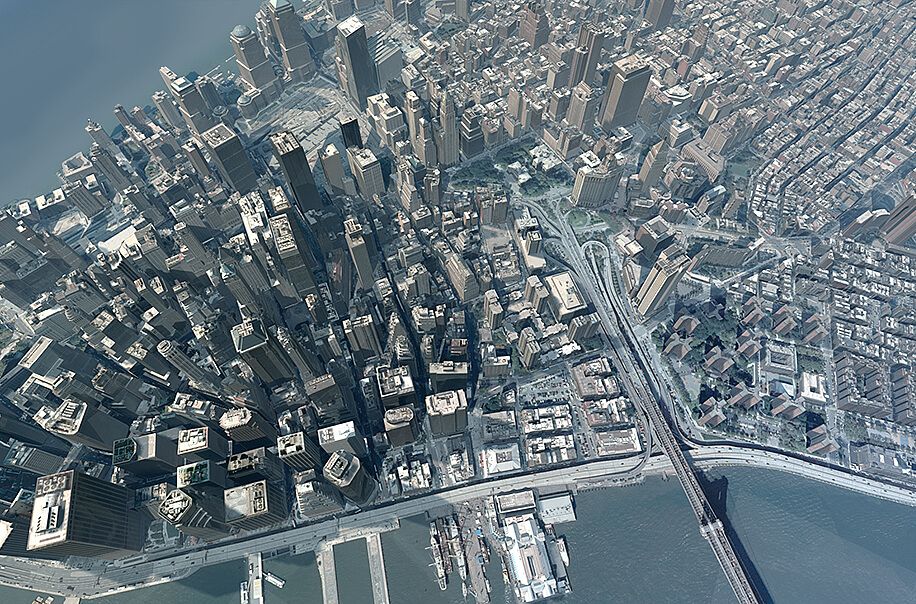
\includegraphics[width=7cm]{U1} }}
    \qquad
    \subfloat[ Vision d'une ville 1]{{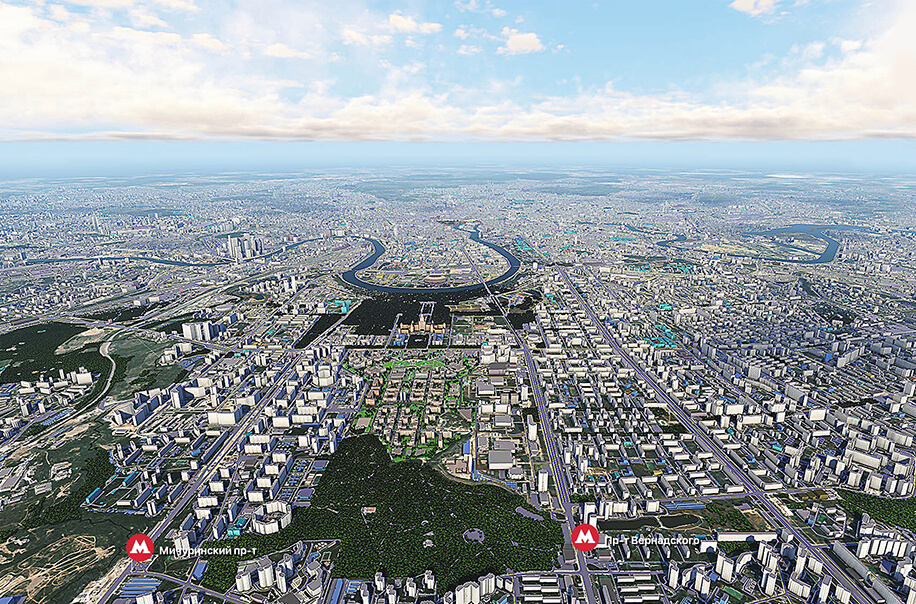
\includegraphics[width=7cm]{U2} }}
    \caption{Moteur de rendu Unigine en mode présentation}
    \label{fig:Ud}
\end{figure}
\FloatBarrier

\begin{figure}[h]
    \centering
    \subfloat[ Simulation d'une centrale]{{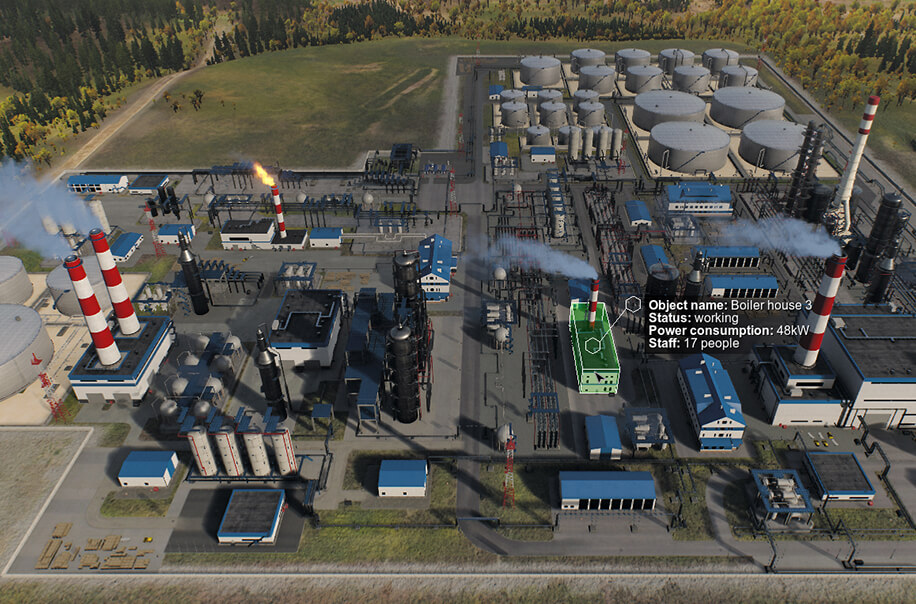
\includegraphics[width=7cm]{U3} }}
    \qquad
    \subfloat[ Simulation de la circulation]{{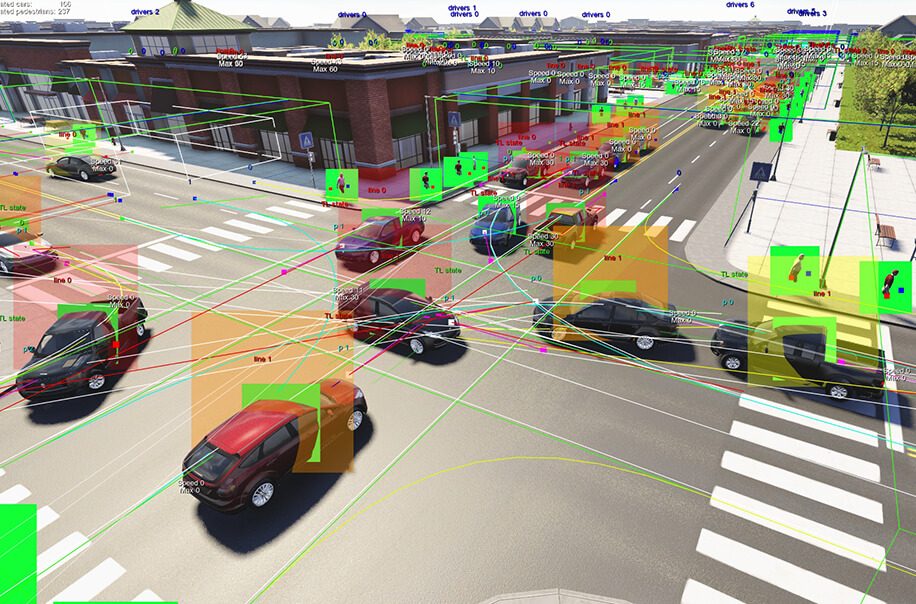
\includegraphics[width=7cm]{U4} }}
    \caption{Moteur de rendu Unigine utilisé pour la simulation}
    \label{fig:U2}
\end{figure}
\FloatBarrier


\section{Conclusion}
Pour conclure, la modélisation 3D et en particulier les maillages 3D jouent un rôle majeur pour le développement des smart cities. En effet, le développement des smart cities nécessitent une représentation 3D particulièrement fidèle à la réalité. De plus, cette représentation doit être suffisamment complexe afin de modéliser des actions et/ou événements hypothétiques. Ainsi, la représentation doit permettre de modéliser les interactions entre les différents composants de la future smart city. Par conséquent, la méthode la plus adaptée est l'acquisition d'un mesh 3d à partir d'une méthode hybride, après avoir construire au préalable un nuage de point (de préférence dense). Pour ce faire, l'usage d'un scanner Lidar est recommandée au sol en raison de sa flexibilité et efficacité d'utilisation. Cela permet en effet d'obtenir un nuage de point au sol précis. Dans un second temps, l'usage de la photogrammétrie pour associer les couleurs des objets au scan laser permettant de modéliser précisément les distances, permettront de construire un nuage de point dense de la vue aérienne de la ville. Enfin, une classification des nuages de points et différents traitements de la donnée permettent de construire un mesh 3D représentatif de la ville.
Finalement, cette représentation fidèle et complexe de la ville permet de visualiser, analyser et simuler différents événements virtuellement tels que la comparaison d'un fort ou faible afflux de personnes et/ou de véhicules, les travaux et leur évolution. Ainsi, ces simulations permises par les modélisation 3D permettront d'anticiper et réduire la consommation d'énergie, la pollution tout en améliorant l'économie et la qualité de vie des habitants grâce à la collecte et l'analyse des données virtuelles. En particulier, les risques d'inondation dans les villes côtières et/ou portuaires peuvent être réduit grâce à un croisement entre les données et propriétés de la ville, et les informations météorologiques locales.



\bibliographystyle{plain} % We choose the "plain" reference style
\bibliography{biblio} % Entries are in the refs.bib file

\end{document}